\documentclass[tikz,border=0.125cm]{standalone}
\begin{document}
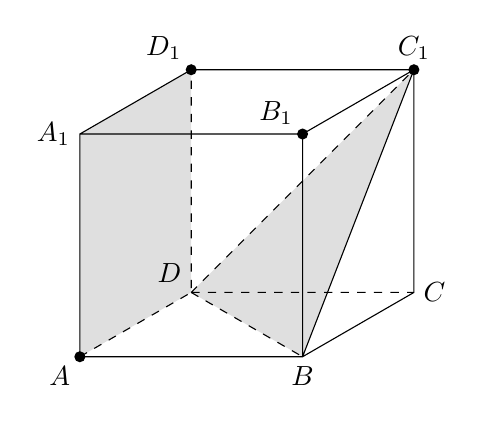
\begin{tikzpicture}[x=(0:2cm), y=(90:2cm*sqrt 2), z=(210:2cm/sqrt 3)]
\foreach \s in {0,1}
  \foreach \l [count=\i from 3, 
    evaluate={\t=-\i*90+45; \n=(\s==0) ? "" : "1";}] in {A,B,C,D}
       \coordinate (\l\n) at (cos \t, \s, sin \t);
%\path (B) -- (C1) coordinate [midway] (E);
\fill [gray!25] (A) -- (D) -- (D1) -- (A1) -- cycle (D) -- (B) -- (C1) -- cycle;
\foreach \p in {A,...,A1,B1,C1,D1} \fill (\p) circle [radius=2pt];
\foreach \p/\a in {A/below left,B/below,C/right,D/above left} \node [\a] at (\p) {$\p$};
\foreach \p/\a in {A/left,B/above left,C/above,D/above left} \node [\a] at (\p1) {$\p_1$};
\draw [dashed] (A) -- (D) -- (D1) (D) -- (C) (D) -- (C1) (D) -- (B);% (D) -- (E);
\draw (A) -- (A1) -- (B1) -- (B)  -- (A) (B) -- (C)  -- (C1) -- (D1) -- (A1) (B) -- (C1) -- (B1);%(E) -- (C);
%\clip (D) -- (E) -- (C);
%\draw [dashed] (E) circle [radius=10pt];
\end{tikzpicture}
\end{document}